% !TEX program = xelatex
\documentclass[12pt,a4paper]{article}
\usepackage[T1]{fontenc}
%\usepackage{tgpagella, eulervm}

% --- XeLatex/LuaLatex ---
\usepackage[no-math]{fontspec}
\IfFontExistsTF{Fira Sans}{
	\setmainfont{Fira Sans}
}

% % --- This is for pdflatex ---
%\usepackage[light, sfdefault]{FiraSans}

\usepackage[italic]{mathastext}
\usepackage[indonesian]{babel}
\usepackage{booktabs}
\usepackage{geometry}
\usepackage{tabularx}
\usepackage{graphicx}
\usepackage{float}
\usepackage{xcolor}
\usepackage{hyperref}
\hypersetup{
	colorlinks=true,  % Colours links instead of boxes
	urlcolor=blue,    % Colour for external hyperlinks
	linkcolor=blue,   % Colour of internal links (sections, etc.)
	citecolor=red,    % Colour of citations
	bookmarks=true,   % Adds PDF bookmarks
	hypertexnames=true
}

\geometry{left=2cm, right=2cm, top=2cm}
\title{\textbf{Panduan Pengamatan Okultasi HIP 35933 oleh Asteroid 1201 Strenua}}
\author{Observatorium Bosscha}
\hyphenation{me-la-ku-kan peng-amat-an deng-an align-ment}
\begin{document}
\maketitle
\noindent\rule{\linewidth}{0.4pt}

\subsection*{Pengantar}
Dokumen ini berisi detail terkait pengambilan data okultasi, baik pada waktu latihan maupun waktu pengamatan sebenarnya.
\subsection*{Langkah 1: Persiapan awal}
\begin{enumerate}
	\item Lakukan persiapan setidaknya \textbf{3 jam} sebelum waktu \textit{event}.
	\item Jika menggunakan NTP timing, pastikan PC/laptop yang digunakan tersinkronisasi dengan server jam atom melalui jaringan internet setidaknya \textbf{2 jam} sebelum waktu pengamatan.
	
	Jika menggunakan GPS, pastikan GPS sudah dalam keadaan \textit{locked} sebelum melakukan pengambilan data.
	\item Pasang instrumen selayaknya pengamatan astronomi secara umum. Lakukan \textit{polar alignment} dan perbaiki \textit{pointing model} jika diperlukan.
	\item Pastikan kapasitas penyimpanan data cukup untuk menyimpan data yang akan diambil. Periksa kembali \textit{setting} pada software pengambilan data (misal SharpCap) untuk memastikan bahwa data akan disimpan dengan format yang benar dan di lokasi yang benar.
	\item Siapkan log--sheet untuk mencatat semua informasi terkait pengamatan, termasuk konfigurasi instrumen, kondisi pengamatan, dan catatan penting lainnya. Isi log-sheet sesuai dengan format yang sudah disediakan. Pastikan semua anggota tim memahami cara mengisi log-sheet dengan benar.
\end{enumerate}
\pagebreak
\subsection*{Langkah 2: \textit{Pointing} ke bintang target}
\begin{enumerate}
	\item Detail bintang target bisa dilihat pada tabel berikut.
	\begin{table}[H]
		\centering
		\large
		\begin{tabular}{ll}
			\toprule
			Target &: HIP 35933, HD 58050  \\
			RA (J2000) &: $7^\mathrm{h} 24^\mathrm{m} 27.648^\mathrm{s}$  \\
			DEC (J2000) &: $15^\circ$ 31' 1.89''  \\
			Waktu \textit{event} &: 12:41.8 UT (lokasi: Obs. Bosscha) \\
			\bottomrule
		\end{tabular}
	\end{table}
	\item Setelah teleskop mengarah ke target, gunakan \textit{finding chart} pada Gambar~\ref{fig:findingchart} untuk memastikan bahwa teleskop sudah benar mengarah ke bintang target. (\underline{catatan:} untuk teleskop yang sudah terkalibrasi dengan baik (\textit{polar aligned}) dan memiliki akurasi pointing tinggi bisa melewati tahap ini).
	\item Pastikan ada bintang lain di sekitar bintang target yang ikut terekam dalam satu \textit{frame}. Bintang ini akan berguna saat ekstraksi data. Bintang target tidak perlu terlalu sempurna berada di tengah \textit{frame}. Minimum FOV dapat dilihat pada Gambar~\ref{fig:findingchart} (kotak merah). 
	\item Pastikan bintang dalam keadaan fokus saat diamati dengan teleskop. Lakukan koreksi jika belum.
\end{enumerate}

\subsection*{Langkah 3: Pengambilan Data}
\begin{enumerate}
	\item Pastikan bintang target berada di tengah \textit{frame} sesaat sebelum pengambilan data. \textcolor{red}{Jangan menggeser bintang target saat pengambilan data meskipun bintang bergeser. Jika \textit{tracking} teleskop kurang baik, pastikan peletakan target dilakukan dengan mempertimbangkan target akan tetap di dalam \textit{frame} selama pengambilan data.} Selama pengambilan data, jangan melakukan \textit{guiding}.
	\item Pastikan \textit{setting} pada SharpCap sudah sesuai dengan Panduan \textit{Setting} Kamera (dokumen terpisah).
	\item Pengambilan data dilakukan \textcolor{blue}{$\sim 5$ menit sebelum waktu okultasi dan dihentikan $\sim 5$ menit setelah waktu okultasi}, dengan detail sebagai berikut.
	\begin{enumerate}
		\item Untuk \textbf{malam latihan}, ambil total 10 menit data dari pukul \textbf{12:37 UT (19:37 WIB)} s.d. \textbf{12:47 UT (19:47 WIB)}.
		
		Gunakan kesempatan ini untuk mencoba-coba waktu \textit{exposure} (dimulai dari nilai rekomendasi) untuk menghasilkan kualitas data dengan SNR yang cukup tanpa mengorbankan terlalu banyak titik sampel (tabel \ref{tab:snrfps}).

\begin{table}[H]
	\centering
	\begin{tabular}{l l l}
		& \textbf{Ideal} & \textbf{Minimum} \\
		\hline
		SNR & $\geq 100$ & 10 \\
		FPS & $\geq 30$ & 5 \\
	\end{tabular}
	\caption{Rekomendasi kualitas data (SNR dan FPS).}
	\label{tab:snrfps}
\end{table}

\item Untuk \textbf{malam gladi}, ambil total 10 menit data dari pukul \textbf{12:37 UT (19:37 WIB)} s.d. \textbf{12:47 UT (19:47 WIB)}.
		
		Kesempatan ini digunakan untuk finalisasi konfigurasi instrumen dan \textit{setting} kamera. Konfigurasi terbaik dari sesi ini akan dipertahankan untuk digunakan pada malam \textit{event}.
		\item Untuk \textbf{malam \textit{event}}, ambil total 10 menit data dari pukul \textbf{12:37 UT (19:37 WIB)} s.d. \textbf{12:47 UT (19:47 WIB)}. 
	\end{enumerate}
	\underline{Catatan umum}: 
	\begin{itemize}
		\item Sesuaikan waktu lokal/waktu zona pengamatan dengan lokasi \textit{chord} masing--masing.
		\item Pantau apakah ada \textit{drop frames}. Catat pada log--sheet jika ada (dan berapa banyak). Catat pula waktu awal dan akhir pengambilan data pada log--sheet.
		\item Gunakan log--sheet yang berbeda untuk setiap malam pengamatan. Beri judul yang sesuai (misal malam latihan, malam gladi, malam \textit{event})
	\end{itemize}
	
%	\pagebreak
	\textbf{DO \& DON'T}
	
	\underline{DO}:
	\begin{itemize}
		\item Kontrol pencahayaan. Lindungi teleskop dari paparan cahaya lingkungan (layar laptop, senter, dll).
	\end{itemize}
	\underline{DON'T}
	\begin{itemize}
		\item Berjalan di sekitar teleskop saat pengambilan data.
		\item Menyalakan senter/lampu saat pengambilan data.		
	\end{itemize} 
\end{enumerate}
\begin{figure}
	\centering
	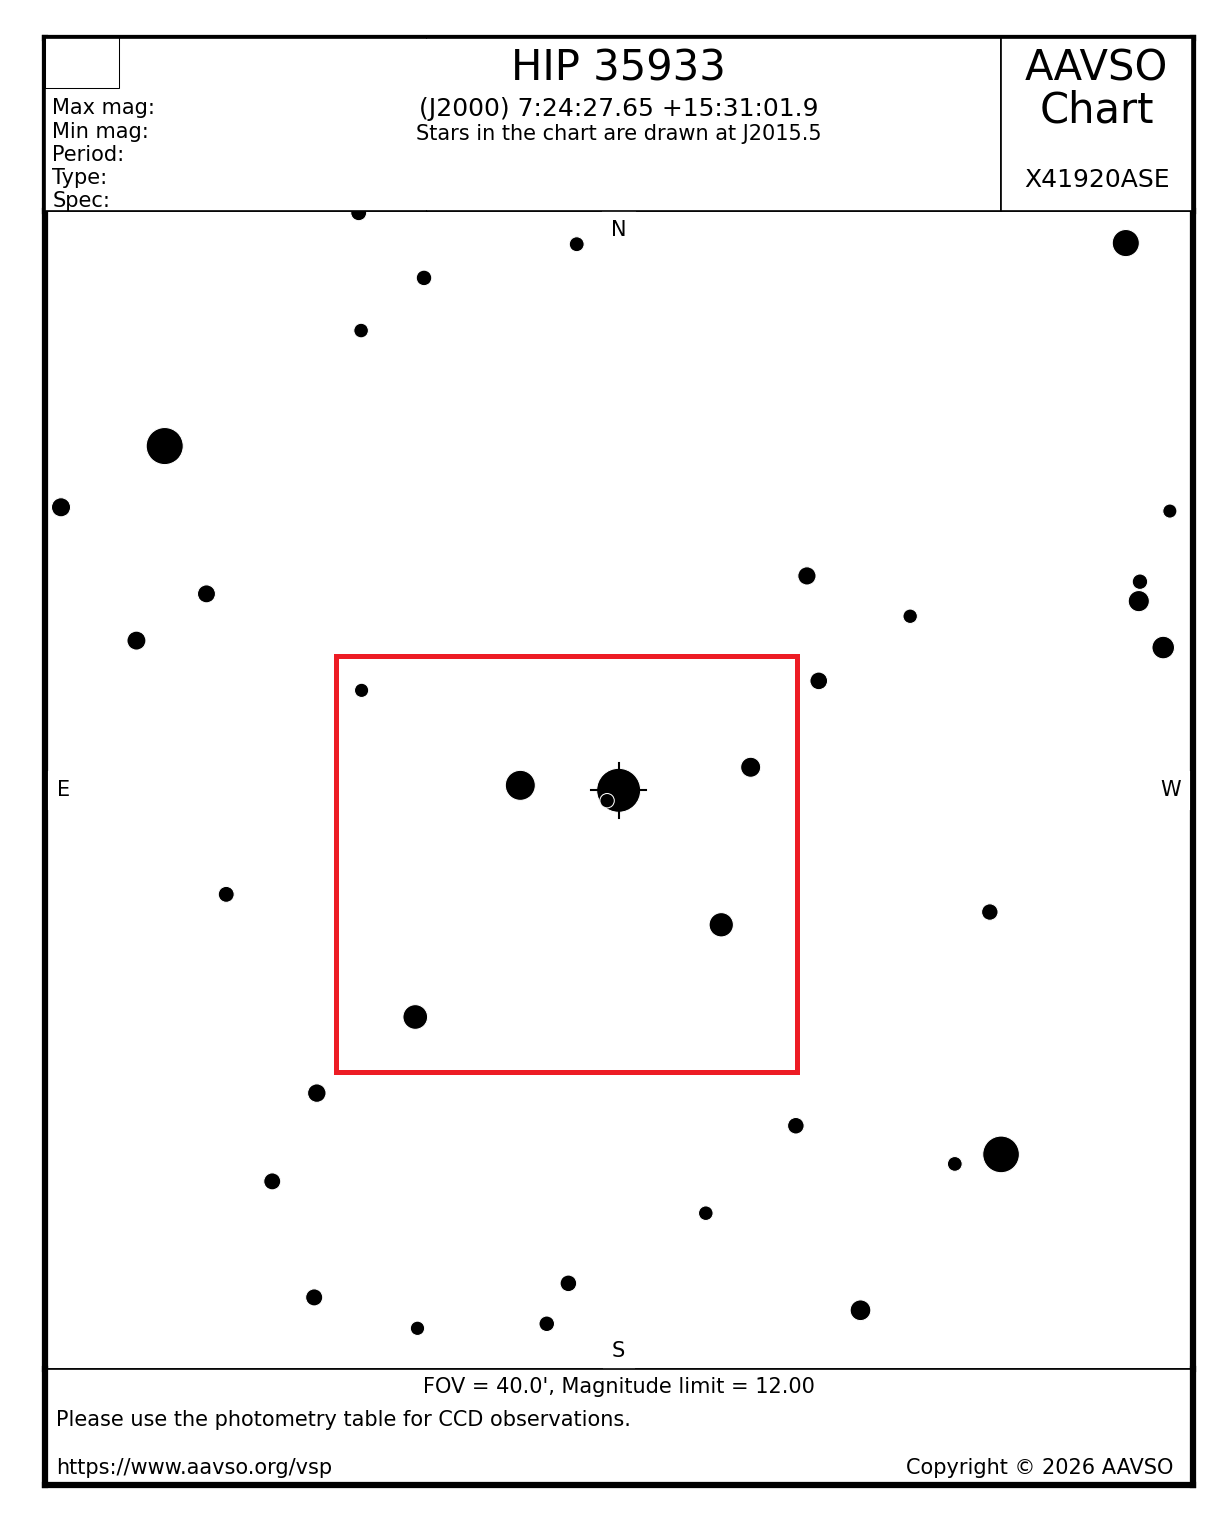
\includegraphics[width=0.65\linewidth]{finding_chart}
	\caption{\textit{Finding chart} untuk bintang target dengan FOV $40' \times 40'$. Kotak merah menunjukkan FOV minimum yang harus tercakup dalam pengamatan. }
	\label{fig:findingchart}
\end{figure}

\subsection*{Langkah 4: Setelah pengamatan}
\begin{enumerate}
	\item Pastikan log--sheet sudah dilengkapi. Tulis semua informasi yang relevan terkait kondisi pengamatan.
	\item Unggah data pengamatan ke tautan yang disediakan sesegera mungkin. Jika pengiriman data tidak memungkinkan dengan menggunakan internet, kontributor dapat mengirimkan data secara fisik ke Observatorium Bosscha. 
	
	Buat folder utama dengan format \textcolor{blue}{\textsc{\textbf{[nama chord]}}} (contoh: \textcolor{blue}{\textbf{BOSSCHA}}). Buat subfolder untuk setiap malam pengamatan dengan format nama folder \textcolor{blue}{\textsc{\textbf{[jenis pengamatan (latihan/gladi/event)]\_[nama chord]\_[tahun bulan tanggal]}}} (contoh: \textcolor{blue}{\textbf{GLADI\_BOSSCHA\_20260401}}) dan masukkan semua data terkait malam pengamatan tersebut ke dalam subfolder yang sesuai. Contoh struktur folder bisa dilihat pada Gambar~\ref{fig:strukturfolder}.
\end{enumerate}
	
\begin{figure}
	\centering
	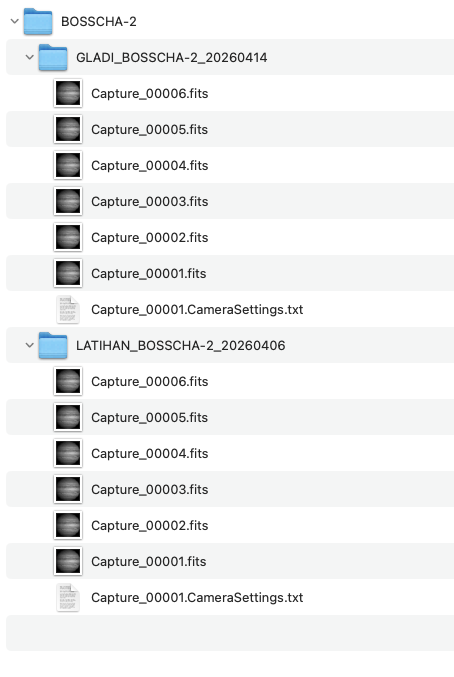
\includegraphics[width=0.65\linewidth]{struktur-folder}
	\caption{Contoh struktur folder untuk pengiriman data.}
	\label{fig:strukturfolder}
\end{figure}
 
\end{document}